\documentclass{article}
\usepackage{tikz}
\usepackage{amsmath}
\begin{document}
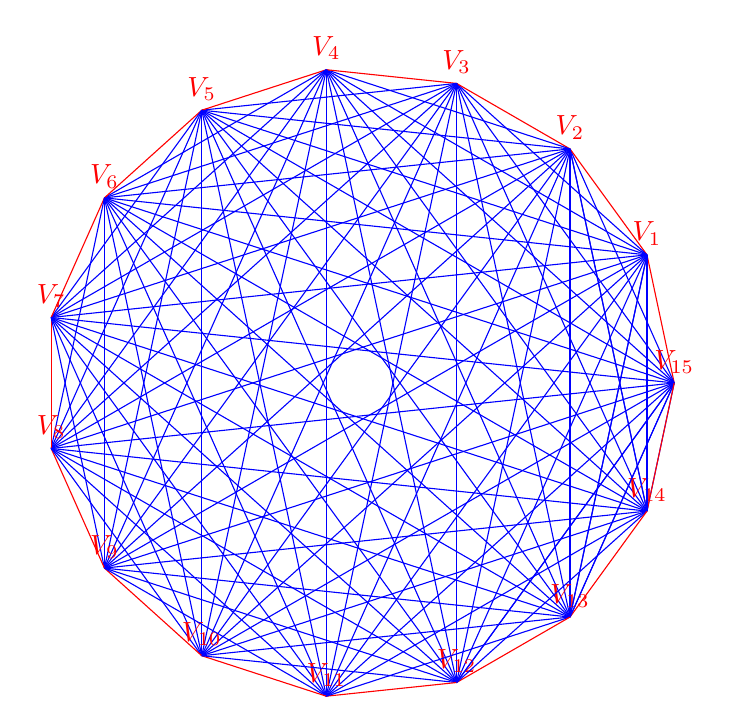
\begin{tikzpicture}[scale = 0.5]
	\pgfmathsetmacro {\n}{15};
	\pgfmathsetmacro{\p}{360/\n};
	\pgfmathsetmacro{\e}{360-\p};
    \foreach \x in {0,\p,...,\e} {
		\pgfmathsetmacro{\a}{int(round((\x + \p)/\p))};
		
        \draw[red] (\x:8cm)  -- (\x+ \p:8cm) node [at end,above] {$V_{\a}$};
		\pgfmathsetmacro{\d}{\x + 2*\p};
		\pgfmathsetmacro{\n}{\x + 3*\p};
			\foreach \y in {\d,\n,...,\e} {
   			     \draw[blue] (\x:8cm) -- (\y:8cm);
										}
					}
\end{tikzpicture}
\end{document}
